\documentclass[../../../../Lectures]{subfiles}


\begin{document}

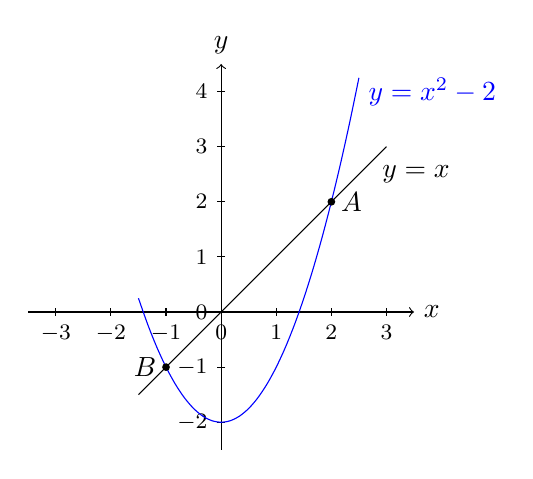
\begin{tikzpicture}[scale=0.7]
    % TODO: LEARN TikZ
    % Currently the code is a copypasta from https://huynhphusi.com/tikz-hinh-phang-gioi-han-boi-3-do-thi/
    \draw[->] (-3.5, 0) -- (3.5, 0) node[right] {$x$};
    \foreach \x in {-3, ..., 3} \draw[shift={(\x,0)}, color=black] (0pt, 2pt) -- (0pt, -2pt) node[below] {\footnotesize $\x$};

    \draw[->] (0, -2.5) -- (0, 4.5) node[above] {$y$};
    \foreach \y in {-2, ..., 4} \draw[shift={(0,\y)}, color=black] (2pt, 0pt) -- (-2pt, 0pt) node[left] {\footnotesize $\y$};

    \draw[domain=-1.5:2.5, smooth, variable=\x, blue] plot ({\x}, {\x * \x - 2});
    \node[right, color=blue] at (2.5, 4){\(y = x^2 - 2\)};

    \draw[domain=-1.5:3, smooth, variable=\x, black] plot ({\x}, {\x});
    \node[right, color=black] at (2.75, 2.5){\(y = x\)};

    \fill (2, 2) circle (2pt) node[right]{\(A\)};
    \fill (-1, -1) circle (2pt) node[left]{\(B\)};
\end{tikzpicture}

\end{document}
